\subsubsection{Vedere le Consuntivazioni per un Progetto}
Dopo essersi autenticati è possibile richiedere la visione delle consuntivazioni effettuate su un determinato progetto scrivendo "ottieni consuntivazione", poi verrà richiesto di inserire il codice del progetto e il chatbot risponderà con un lungo messaggio contenente tutte le consuntivazioni effettuate, al momento della stesura di questo documento non è possibile filtrare le consuntivazioni per un dato per periodo. 
\begin{figure}[H]
    \centering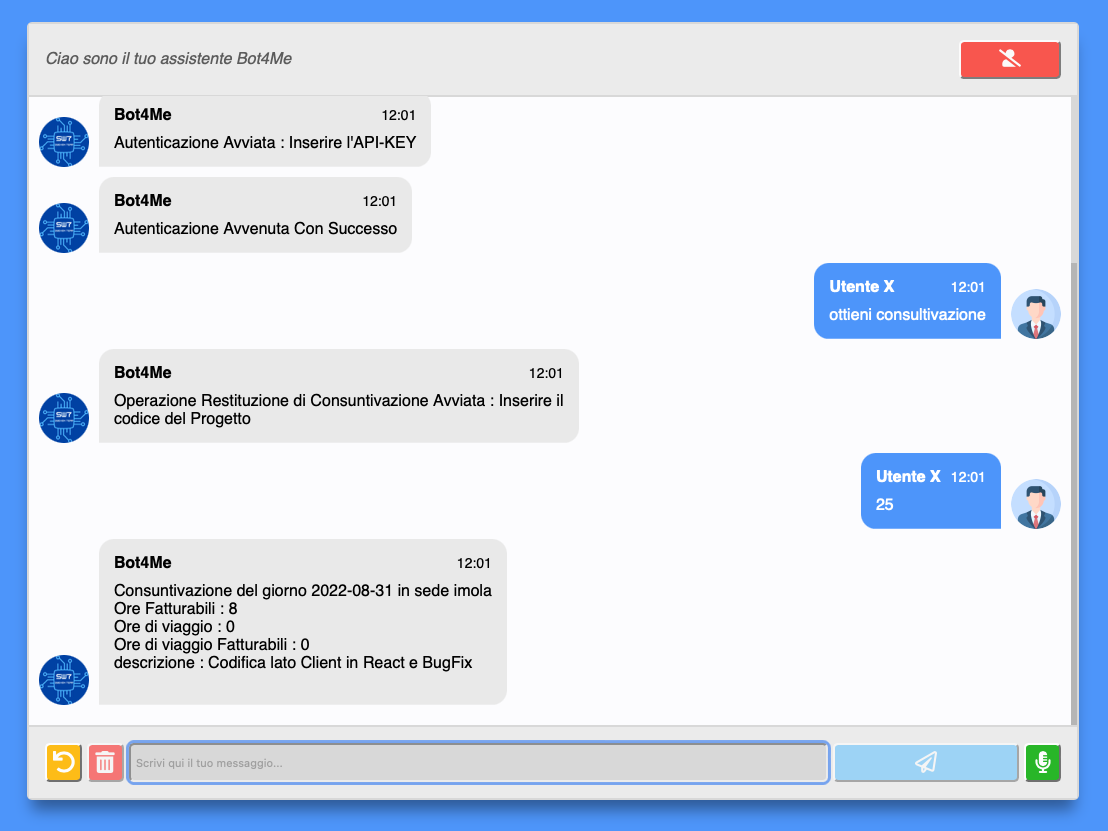
\includegraphics[width=0.9\textwidth, height=0.7\textheight, keepaspectratio]{images/schermata_ottieni_consultivazione.png}
    \caption{Schermata Dialogo Ottenimento Consuntivazioni Registrate per Progetto}
\end{figure}